\documentclass[
  coursecode={APSC 171},
  assignmentname={Week 6 Material - Defining and Estimating Integrals as Areas},
  solutiontitle=Solution,
  nodate,
  draft,
  % final,
]{
  ltxanswer%
}

\usepackage{bch-style}

\sisetup{per-mode=symbol}

\pgfplotsset{compat=newest}
\pgfplotsset{
  integral/.style={
    domain=0:pi/2,
    samples=5,
  },
  integral fill/.style={
    integral,
    draw=none,
    fill=#1,
    on layer=axis background,
  },
  integral fill/.default=blue!5,
  integral line/.style={
    integral,
    draw=#1
  },
  integral line/.default=black,
}

\begin{document}
  \begin{questions}
    \setcounter{question}{24}
    \question{}\
    \begin{parts}
      \part{}
      \begin{solution}
        Let \(D_{\text{right}}\) denote distance travelled by the car as estimated by the right sum. Then the right sum, in terms of \(t\) and \(v(t)\), can be calculated using
        \begin{align*}
          D_{\text{right}} &= RIGHT(5)                                                          \\
                           &= \Delta t \sum_{i=1}^{5} v(t_{i})\numberthis\label{eq:right-sum-a}
        \end{align*}
        From the table, it can be observed that the width of each subinterval is \qty{0.2}{\hour}. Otherwise, here's the calculation for completeness:
        \begin{align*}
          \Delta t &= \frac{b-a}{n}    \\
                   &= \frac{1-0}{5}    \\
                   &= \qty{0.2}{\hour}
        \end{align*}
        Then let's use~\eqref{eq:right-sum-a} to calculate the estimated distance:
        \begin{align*}
          D_{\text{right}} &= \Delta t \sum_{i=1}^{5} v(t_{i}) \\
                           &= 0.2 (30 + 30 + 70 + 90 + 90)     \\
          \alignedbox{     &= \qty{62}{\km}}
        \end{align*}
      \end{solution}

      \part{}
      \begin{solution}
        Let \(G_{\text{right}}\) denote the amount of gas consumed by the car as estimated by and let \(g(v(t))\) be the fuel gas efficiency of the car given a speed \(v(t)\).

        Unit analysis: We want \unit{\litre} from the distances (speed \(\times\) time) in part~(\ref{part@25@1}) and the efficiency from the table.
        \begin{equation*}
          \underbrace{\cancel{\unit{\hour}}}_{t} \times \underbrace{\frac{\cancel{\unit{\km}}}{\cancel{\unit{\hour}}}}_{v(t)} \times \underbrace{\frac{\unit{\litre}}{\qty{100}{\cancel\km}}}_{g(v(t))} = \frac{1}{100} \unit{\litre}
        \end{equation*}
        So then the terms we're summing over are \(f(t_{i}) = v(t_{i})g(v(t_{i}))\), which implies that the quantity that we're looking for is
        \begin{align*}
          G_{\text{right}} &= RIGHT(5)                                                                      \\
                           &= \Delta t \sum_{i=1}^{5} f(t_{i})                                              \\
                           &= \Delta t \sum_{i=1}^{5} v(t_{i})g(v(t_{i})).\numberthis\label{eq:right-sum-b}
        \end{align*}
        With \(\Delta t\) as before, using~\eqref{eq:right-sum-b} to calculate the estimated gas consumed yields
        \begin{align*}
          G_{\text{right}} &= \Delta t \sum_{i=1}^{5} v(t_{i})g(v(t_{i}))                                                                                                    \\
                           &= 0.2 \biggl(30 \cdot \frac{15}{100} + 30 \cdot \frac{15}{100} + 70 \cdot \frac{7}{100} + 90 \cdot \frac{8}{100} + 90 \cdot \frac{8}{100}\biggr) \\
          \alignedbox{     &= \qty{5.66}{\litre}}
        \end{align*}
      \end{solution}
    \end{parts}

    \question{}\
    \begin{parts}
      \part{}
      \begin{solution}
        The length of each of the four subintervals is
        \begin{align*}
          \Delta x &= \frac{b-a}{n}             \\
                   &= \frac{\frac{\pi}{2}-0}{4} \\
                   &= \frac{\pi}{8}
        \end{align*}
        With \(f(x)=\cos(x)\) and \(n=4\), the trapezoidal rule gives us
        \begin{align*}
          \int_{0}^{\frac{\pi}{2}} f(x) \dl3 x &\approx TRAP(4)                                                                                                                                                   \\
                                               &= \Delta x \left(\frac{f(x_{0}) + f(x_{4})}{2} + \sum_{i=1}^{3} f(x_{i})\right)                                                                                   \\
                                               &= \frac{\pi}{8} \left(\frac{\cos(0) + \cos(\frac{\pi}{2})}{2} + \cos\Bigl(\frac{\pi}{8}\Bigr)+\cos\Bigl(\frac{\pi}{4}\Bigr)+\cos\Bigl(\frac{3\pi}{8}\Bigr)\right) \\
          \alignedbox{                         &\approx 0.987}
        \end{align*}
      \end{solution}

      \newpage

      \part{}
      \begin{solution}
        \begin{answerfigure}
          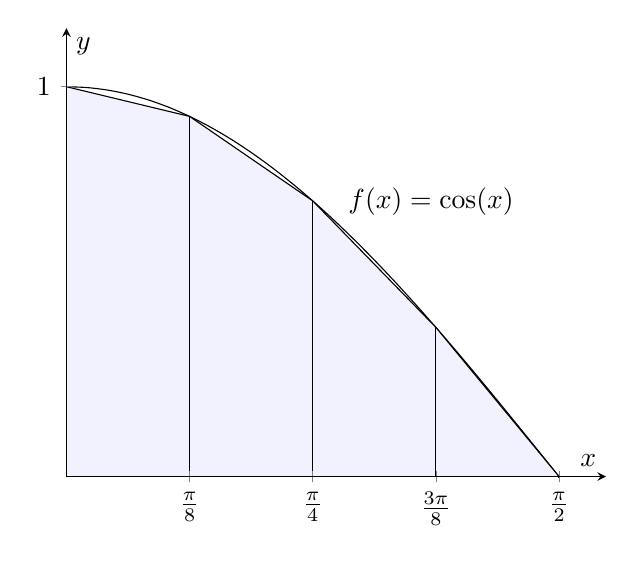
\begin{tikzpicture}[
              declare function={f=cos(deg(x));},
            ]
            \begin{axis}[
                xtick={0.3927, 0.7854, 1.1781, 1.5708},
                xticklabels={\(\frac{\pi}{8}\), \(\frac{\pi}{4}\), \(\frac{3\pi}{8}\), \(\frac{\pi}{2}\)},
                ytick={0,...,1},
                xlabel={\(x\)},
                xmin=0,
                xmax=pi/2+0.15,
                ylabel={\(y\)},
                ymin=0,
                ymax=1.15,
                enlargelimits=true,
                axis lines=middle,
                clip=false,
                domain=0:pi/2,
                axis on top,
              ]

              \addplot [smooth, domain=0:pi/2] {f} node[pos=0.5, above right] {\(f(x)=\cos(x)\)};
              % The filled area under the approximate integral
              \addplot [integral fill] {f} \closedcycle;
              % The approximate integral
              \addplot [integral line=black] {f};
              % The vertical lines between the segments
              \addplot [integral, ycomb] {f};
            \end{axis}
          \end{tikzpicture}
          \caption{A \sout{sketch} graph of the trapezoidal rule for approximating the integral of \(\cos(x)\) from \(0\) to \(\frac{\pi}{2}\).}\label{fig:trapezoidal-rule-cos}
        \end{answerfigure}
        From Figure~\ref{fig:trapezoidal-rule-cos}, we can deduce that the estimate from part~(\ref{part@26@1}) is an \textbf{underestimate} of the exact integral value.
      \end{solution}
    \end{parts}
  \end{questions}
\end{document}
